\section{A família Pattern}

Vamos tentar algo diferente agora. Digite e rode esta linha de código:

\begin{lstlisting}[style=SuperCollider-IDE, basicstyle=\scttfamily\footnotesize]
Pbind(\degree, Pseries(0, 1, 30), \dur, 0.05).play;
\end{lstlisting}

\subsection{Conheça o Pbind}

\texttt{Pbind} é um membro da família Pattern ("padrão") no SuperCollider. O P maiúsculo no \texttt{Pbind} e \texttt{Pseries} remete a \emph{Pattern}; conheceremos outros membros da família em breve. Por ora, veremos mais de perto somente o \texttt{Pbind}. Experimente este exemplo reduzido ao mínimo:

\begin{lstlisting}[style=SuperCollider-IDE, basicstyle=\scttfamily\footnotesize]
Pbind(\degree, 0).play;
\end{lstlisting}

A única coisa que esta linha de código faz na vida é tocar a nota \emph{dó central}, uma vez por segundo. A palavra-chave \texttt{\textbackslash degree} se refere a graus de uma escala e o número 0 representa o primeiro grau da escala (uma escala de Dó Maior é subentendida, então esta é a própria nota dó). Note que o SuperCollider começa a contar as coisas do 0 e não do 1. Em uma linha simples como esta acima, as notas dó, ré, mi, fá, sol\dots seriam representadas pelos números 0, 1, 2, 3, 4\dots Tente mudar o número e perceba como a nota muda quando você reexecuta. Você também pode escolher notas abaixo do dó central (por exemplo, -2 nos dá a nota lá abaixo do dó central). Resumindo, apenas imagine que o dó central do piano é 0 e conte teclas brancas para cima ou para baixo (números positivos ou negativos) para conseguir qualquer outra nota.

Agora brinque um pouco com a duração das notas. \texttt{Pbind} usa a palavra-chave \texttt{\textbackslash dur} para especificar durações em segundos:

\begin{lstlisting}[style=SuperCollider-IDE, basicstyle=\scttfamily\footnotesize]
Pbind(\degree, 0, \dur, 0.5).play;
\end{lstlisting}

Claro que isso ainda é muito rígido e inflexível---sempre a mesma nota, sempre a mesma duração. Não se preocupe: as coisas vão melhorar muito em breve.
\subsection{Pseq}

Vamos lá e toquemos várias notas na sequência, como uma escala. Vamos também deixar nossas notas mais curtas, digamos, com duração de 0.2 segundos.
 
\begin{lstlisting}[style=SuperCollider-IDE, basicstyle=\scttfamily\footnotesize]
Pbind(\degree, Pseq([0, 1, 2, 3, 4, 5, 6, 7], 1), \dur, 0.2).play;
\end{lstlisting}

Esta linha introduz um novo membro da família Pattern: \texttt{Pseq}. Como o nome poderia sugerir, este Pattern lida com sequências. Tudo que um \texttt{Pseq} precisa para tocar uma sequência é:
\begin{itemize}
\item uma lista de itens entre colchetes
\item um número de repetições.
\end{itemize} 

No exemplo, a lista é \texttt{[0, 1, 2, 3, 4, 5, 6, 7]} e o número de repetições é \texttt{1}. Este \texttt{Pseq} simplesmente diz: "toque uma vez todos os itens da lista, na sequência." Perceba que estes dois elementos, lista e número de repetições, estão dentro dos parênteses que pertencem ao \texttt{Pseq} e são separados por uma vírgula.

Também perceba onde o \texttt{Pseq} aparece no interior do \texttt{Pbind}: é o valor de entrada de \texttt{\textbackslash degree}. Isso é importante: em vez de fornecer um número único e fixo para o grau da escala (como no nosso primeiro \texttt{Pbind} simples), \emph{estamos fornecendo todo um Pseq: uma receita para uma sequência de números}. Com isto em mente, podemos facilmente expandir esta ideia e usar outra Pseq para controlar também as durações.
 
\begin{lstlisting}[style=SuperCollider-IDE, basicstyle=\scttfamily\footnotesize]
Pbind(\degree, Pseq([0, 1, 2, 3, 4, 5, 6, 7], 5), \dur, Pseq([0.2, 0.1, 0.1, 0.2, 0.2, 0.35], inf)).play;
\end{lstlisting}
 
O que está acontecendo neste exemplo? Primeiro, mudamos o número de repetições do primeiro \texttt{Pseq} para 5, de modo que toda a escala vai tocar cinco vezes. Segundo, substituímos o valor antes fixo de 0.2 de \texttt{\textbackslash dur} por um outro \texttt{Pseq}. Este novo \texttt{Pseq} tem uma lista de seis itens: \texttt{[0.2, 0.1, 0.1, 0.2, 0.2, 0.35]}. Estes números se tornam valores de duração das notas resultantes. O valor de \texttt{repeats} deste segundo \texttt{Pseq} é definido como \texttt{inf}, que quer dizer "infinito". Isso sgnifica que o \texttt{Pseq} não tem limite no número de vezes que ele pode repetir esta sequência. Então o \texttt{Pbind} toca para sempre? Não: ele para depois que o \emph{outro} \texttt{Pseq} terminou seu trabalho, isto é, depois que a sequência de graus de escala foi tocada 5 vezes.

Finalmente, o exemplo tem um total de oito notas diferentes (a lista no primeiro \texttt{Pseq}), enquanto há apenas seis valores para duração (segundo \texttt{Pseq}). Quando você fornece sequências de tamanhos diferentes como estas, o \texttt{Pbind} simplesmente as faz circular o quanto for preciso.

Responda estas perguntas para praticar o que você aprendeu:
\begin{itemize}
\item Experimente o número 1 em vez de inf como o argumento \texttt{repeats} do segundo \texttt{Pseq}. O que acontece?
\item Como você pode fazer este Pabind tocar para sempre?
\end{itemize}

Soluções estão no final do livro.\endnote{Primeira pergunta: quando você usa o número 1 em vez de \texttt{inf} como o argumento \texttt{repeats} do segundo \texttt{Pseq}, o Pbind para depois que 6 notas foram tocadas (isto é, depois que uma sequência completa de valores de duração foi tocada). Segunda questão: para fazer o Pbind tocar para sempre, simplesmente use \texttt{inf} como valor para \texttt{repeats} em todos os Patterns internos.}

\subsection{Deixe seu código mais legível}

Você deve ter percebido que a linha de código acima é um tanto longa. De fato, ela é tão longa que quebra em uma nova linha, mesmo que tecnicamente se trate de um enunciado único. Linhas de código longas podem ser confusas de ler. Para evitar isso, é uma prática comum quebrar o código em várias linhas indentadas; com o objetivo de torná-lo o mais claro e inteligível possível. O mesmo \texttt{Pbind} pode ser escrito assim:

\begin{lstlisting}[style=SuperCollider-IDE, basicstyle=\scttfamily\footnotesize]
(
Pbind(
	\degree, Pseq([0, 1, 2, 3, 4, 5, 6, 7], 5),
	\dur, Pseq([0.2, 0.1, 0.1, 0.2, 0.2, 0.35], inf)
).play;
)
\end{lstlisting}

De agora em diante, adquira o hábito de escrever seus \texttt{Pbind}s deste jeito. Escrever código com uma aparência arrumada e bem organizada vai ajudá-lo bastante no aprendizado do SuperCollider.

Além disso, perceba que envolvemos este \texttt{Pbind} dentro de parênteses para criar um bloco de código (lembra-se da seção \ref{sec:code-block}?): como ele não está mais em uma única linha, precisamos fazer isso para conseguir rodá-lo todo de uma vez. Apenas tenha certeza que o cursor esteja em algum lugar no interior do bloco antes de executá-lo.


\subsection{Quatro maneiras de especificar alturas}

\texttt{Pbind} aceita outras maneiras de especificar alturas, não apenas graus de escala.
\begin{itemize}
\item Se você quiser usar todas as doze notas cromáticas (teclas brancas e pretas do piano), você pode usar \texttt{\textbackslash note} em vez de \texttt{\textbackslash degree}. 0 continuará representando o dó central, mas agora os números incluem as teclas pretas do piano (0=dó central, 1=dó$\sharp$, 2=ré, etc).
\item Se você preferir usar a numeração de notas MIDI, use \texttt{\textbackslash midinote} (60=dó central, 61=dó$\sharp$, 62=ré, etc).
\item Finalmente, se você quiser especificar frequências diretamente em Herz, use \texttt{\textbackslash freq}.
\end{itemize}

Veja a figura \ref{fig:scale-degrees} para uma comparação dos quatro métodos.

\begin{figure}[h]
\centering
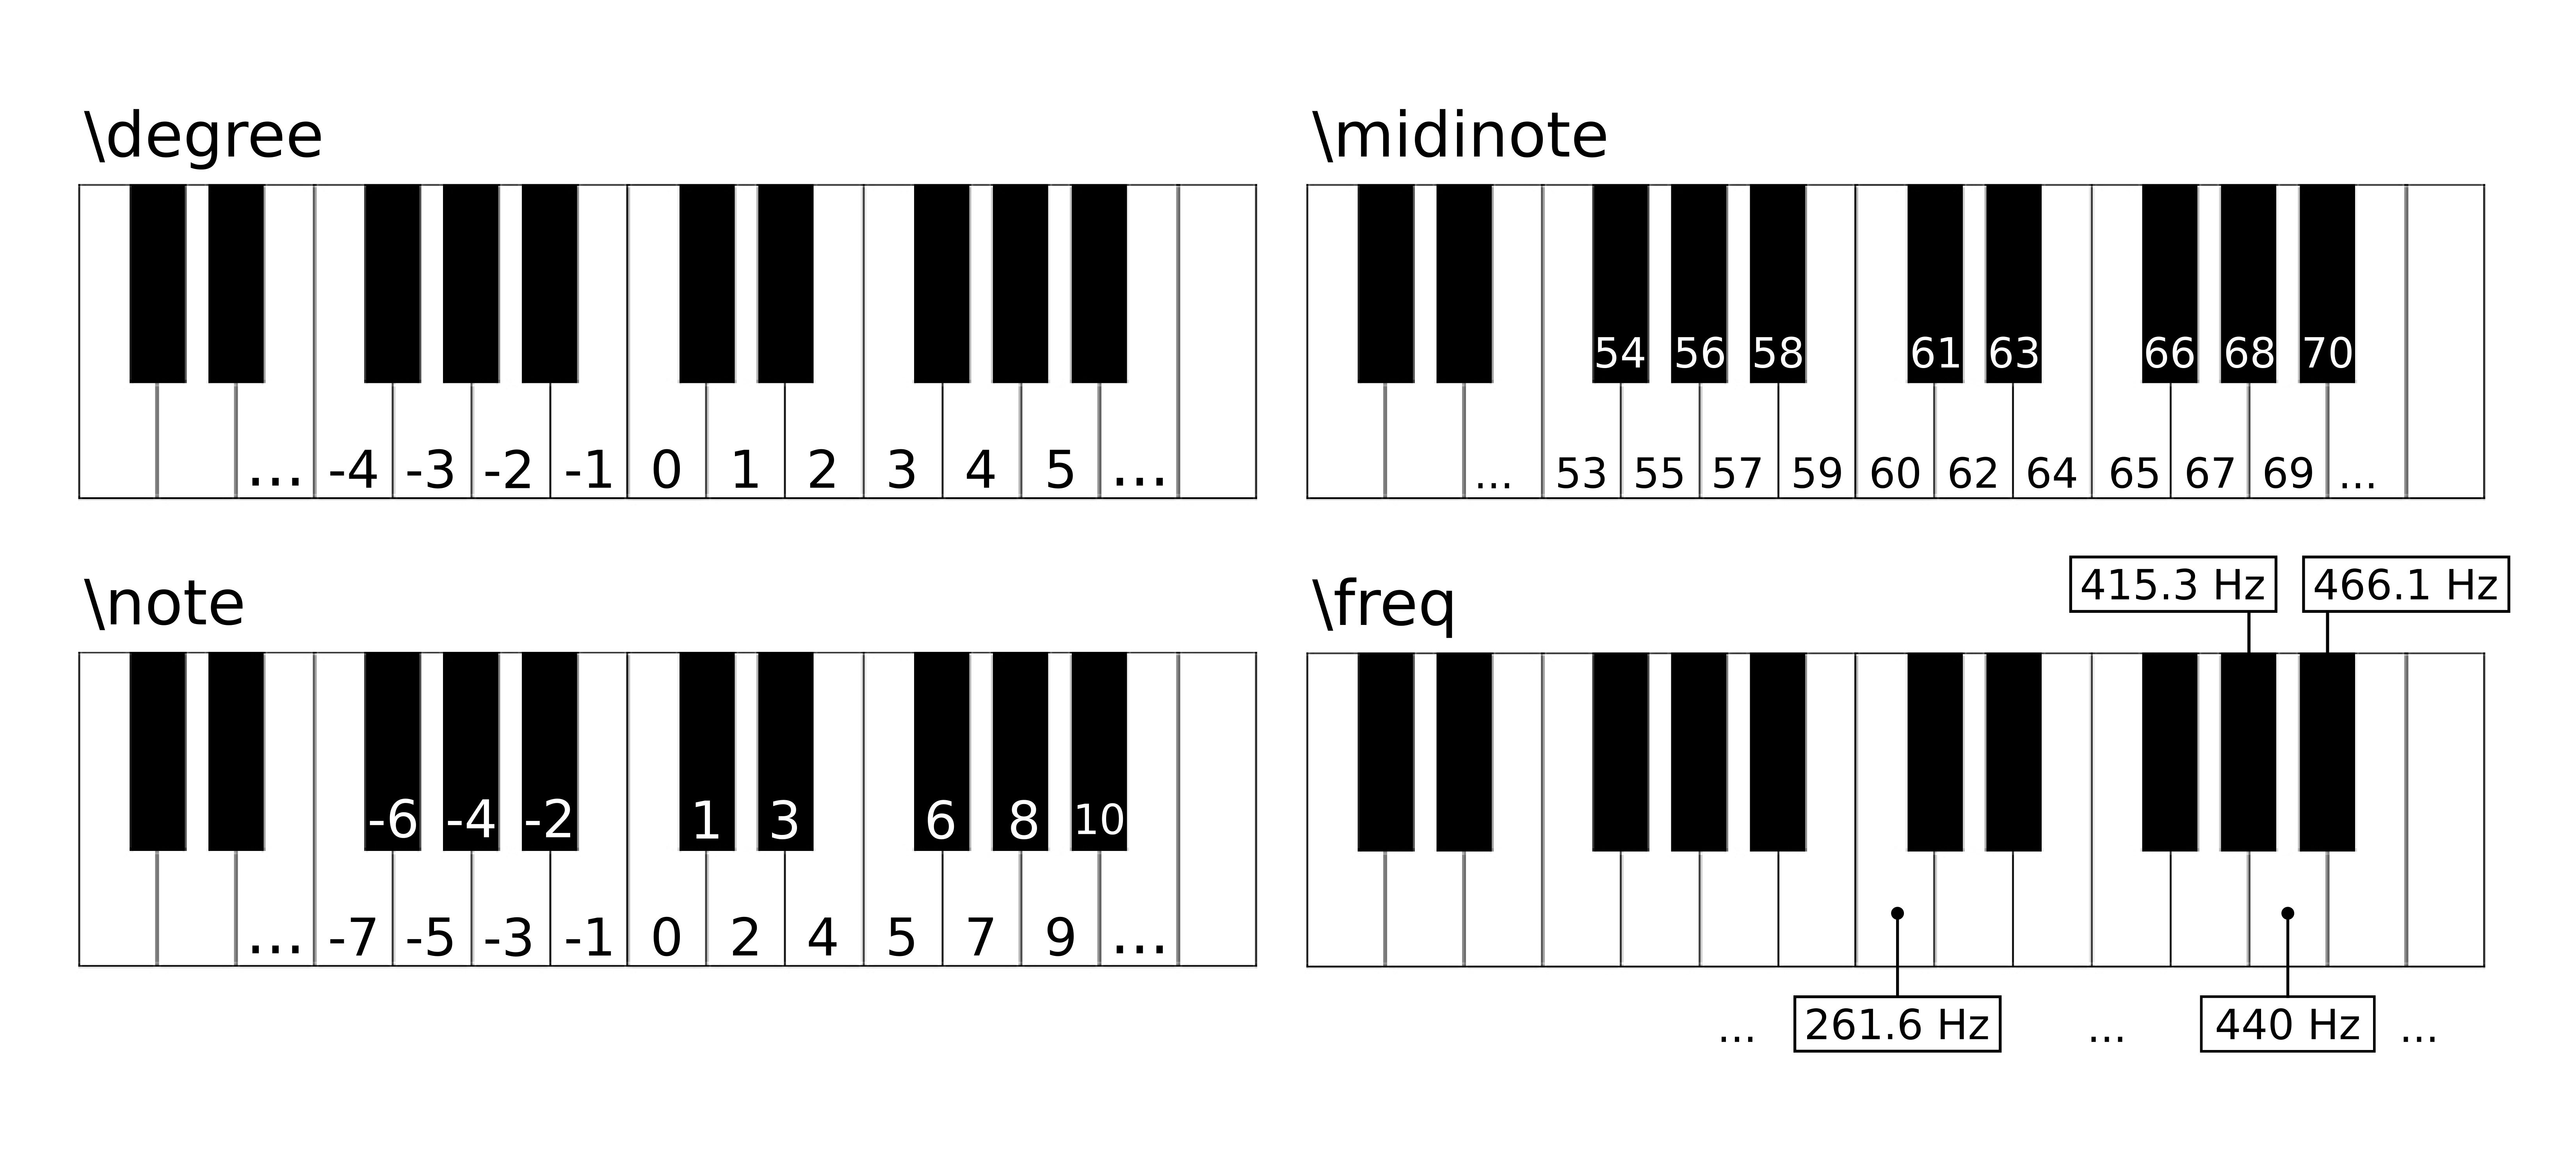
\includegraphics[scale=0.4]{fig-piano-keyboard-degree-note-midinote-freq.png}
\caption{Comparando graus de escala, números de nota, notas MIDI e frequências}
\label{fig:scale-degrees}
\end{figure}

No próximo exemplo, os quatro Pbinds vão tocar a mesma nota: o lá acima do dó central (lá 4).

\begin{lstlisting}[style=SuperCollider-IDE, basicstyle=\scttfamily\footnotesize]
Pbind(\degree, 5).play;
Pbind(\note, 9).play;
Pbind(\midinote, 69).play;
Pbind(\freq, 440).play;
\end{lstlisting}


\bigskip
\todo[inline, color=green!40]{
DICA: Lembre-se que cada maneira de especificar alturas espera números em âmbitos sensivelmente diferentes. Uma lista de números como \texttt{[-1, 0, 1, 3]} faz sentido para \texttt{\textbackslash degree} e \texttt{\textbackslash note}, mas não faz sentido para \texttt{\textbackslash midinote} ou \texttt{\textbackslash freq}. A tabela abaixo compara alguns valores usando o teclado do piano como referência.
}
\bigskip


\begin{tabular}{|l|c|c|c|c|c|}
\hline 
  & \textbf{lá 0 (nota mais grave do piano)} & \textbf{dó 4} & \textbf{lá 4} & \textbf{dó 5} & \textbf{dó 8 (nota mais aguda do piano)} \\ 
\hline 
\texttt{\textbackslash degree} & -23 & 0 & 5 & 7 & 21 \\
\hline
\texttt{\textbackslash note} & -39 & 0 & 9 & 12 & 48 \\
\hline
\texttt{\textbackslash midinote} & 21 & 60 & 69 & 72 & 108 \\
\hline
\texttt{\textbackslash freq} & 27.5 & 261.6 & 440 & 523.2 & 4186 \\
\hline
\end{tabular}
\bigskip


\subsection{Mais palavras-chaves: amplitude e legato}

O novo exemplo introduz duas novas palavras-chaves: \texttt{\textbackslash amp} e \texttt{\textbackslash legato}, que definem a amplitude dos eventos e a quantidade de legato entre as notas. Perceba como o código fica bem mais fácil de ler, graças a uma boa indentação e distribuição em diversas linhas. Parênteses externos (no topo e embaixo) são usados para delimitar um bloco de código a ser rapidamente excutado.

 
\begin{lstlisting}[style=SuperCollider-IDE, basicstyle=\scttfamily\footnotesize]
(
Pbind(
	\degree, Pseq([0, -1, 2, -3, 4, -3, 7, 11, 4, 2, 0, -3], 5),
	\dur, Pseq([0.2, 0.1, 0.1], inf),
	\amp, Pseq([0.7, 0.5, 0.3, 0.2], inf),
	\legato, 0.4
).play;
)
\end{lstlisting}
 

\texttt{Pbind} tem muitas destas palavras-chaves pré-definidas e com o tempo você aprenderá mais delas. Por agora, vamos nos centrar em apenas algumas---uma para altura (escolha entre \texttt{\textbackslash degree}, \texttt{\textbackslash note}, \texttt{\textbackslash midinote} ou \texttt{\textbackslash freq}), uma para durações (\texttt{\textbackslash dur}), uma para amplitude (\texttt{\textbackslash amp}) e uma para legato (\texttt{\textbackslash legato}). Durações estão em tempos (neste caso, 1 batida por segundo, que é o padrão); a amplitude deve estar entre 0 e 1 (0 = silêncio, 1 = muito alto); e o legato funciona melhor com valores entre 0.1 e 1 (se você não tem certeza o que o legato faz, simplesmente experimente o exemplo acima com 0.1, depois 0.2, depois 0.3, até chegar no 1 e ouça os resultados).

Tome o último exemplo como um  ponto de partida e crie novos \texttt{Pbind}s. Mude a melodia. Introduza novas listas de durações e amplitudes. Experimente usar \texttt{\textbackslash freq} para alturas. Lembre, você sempre pode usar um número fixo para qualquer um destes parâmetros, se é o que você precisa. Por exemplo, se você quer que todas as notas da sua melodia tenham 0.2 segundos de duração, não há porque escrever \texttt{Pseq[0.2, 0.2, 0.2, 0.2\dots}, nem mesmo \texttt{Pseq([0.2], inf)}---simplesmente remova toda a estrutura do \texttt{Pseq} e escreva 0.2 no lugar.

\subsection{Prand}

\texttt{Prand} é um primo próximo do \texttt{Pseq}. Ele também aceita uma lista e um número de repetições. Mas em vez de ir tocando a lista na sequência, \texttt{Prand} \emph{escolhe um item aleatório da lista a cada vez}. Experimemnte:

 
\begin{lstlisting}[style=SuperCollider-IDE, basicstyle=\scttfamily\footnotesize]
(
Pbind(
	\degree, Prand([2, 3, 4, 5, 6], inf),
	\dur, 0.15,
	\amp, 0.2,
	\legato, 0.1
).play;
)
\end{lstlisting}
 

Substitua \texttt{Prand} pelo \texttt{Pseq} e compare os resultados. Agora experimente usar \texttt{Prand} para durações, amplitudes e legato.

\subsection{Pwhite}

Outro membro popular da família Pattern é o \texttt{Pwhite}. É um gerador de números aleatórios de distribuição uniforme (o nome vem de "white noise", ruído branco). Por exemplo, \texttt{Pwhite(100, 500)} irá fornecer números aleatórios entre 100 e 500.
 
\begin{lstlisting}[style=SuperCollider-IDE, basicstyle=\scttfamily\footnotesize]
(
Pbind(
	\freq, Pwhite(100, 500),
	\dur, Prand([0.15, 0.25, 0.3], inf),
	\amp, 0.2,
	\legato, 0.3
).trace.play;
)
\end{lstlisting}
 

O exemplo acima também mostra outro truque útil: a mensagem \texttt{trace} logo antes de \texttt{play}. Isso imprime na Post window os valores selecionados para cada evento. Muito útil para corrigir problemas ou simplesmente para entender o que está acontecendo!

Preste atenção nas diferenças entre \texttt{Pwhite} e \texttt{Prand}: mesmo que ambos tenham a ver com aleatoriedade, eles aceitam argumentos distintos e fazem coisas diferentes. Dentro dos parênteses do \texttt{Pwhite} você só precisa fornecer um limite mínimo e máximo: \texttt{Pwhite(mínimo, máximo)}. Números aleatórios serão escolhidos no interior deste âmbito. \texttt{Prand}, por outro lado, aceita uma lista de itens (necessariamente entre colchetes) e um número de repetições: \texttt{Prand([lista, de, itens], repetições)}. Itens aleatórios serão escolhidos \emph{desta lista}.

Explore ambos e garanta que você entendeu completamente a diferença.


\bigskip
\todo[inline, color=green!40]{ 
DICA: Um \texttt{Pwhite} com dois números inteiros vai apenas gerar inteiros. Por exemplo, \texttt{Pwhite(100, 500)} vai gerar números como 145, 568, 700, mas não 145.6, 450.32, etc. Se você quer números decimais na sua saída, escreva \texttt{Pwhite(100, 500.0)}. Isso é muito útil para, digamos, amplitudes: se você escreve \texttt{Pwhite(0, 1)} vai obter apenas 0 ou 1, mas escreva \texttt{Pwhite(0, 1.0)} e você terá todos os resultados intermediários.
}
\bigskip
 


Tente as seguintes perguntas para testar seu novo conhecimento:

\begin{enumerate}[a)]
\item Qual a diferença entre os resultados de \texttt{Pwhite(0, 10)} e \texttt{Prand([0, 4, 1, 5, 9, 10, 2, 3], inf)}?

\item Se você precisa de um fluxo de números inteiros escolhidos aleatoriamente entre 0 e 100, você poderia usar um \texttt{Prand}?

\item Qual a diferença entre os resultados de \texttt{Pwhite(0, 3)} e \texttt{Prand([0, 1, 2, 3], inf)}? E se você escrever \texttt{Pwhite(0, 3.0)}?

\item  Rode os exemplos abaixo. Usamos \texttt{\textbackslash note} em vez de \texttt{\textbackslash degree} para tocar uma escala de dó menor (que inclui teclas pretas). A lista \texttt{[0, 2, 3, 5, 7, 8, 11, 12]} tem oito números dentro dela, correspondendo às notas dó, ré, mi$\flat$, fá, sol, lá$\flat$, si, dó, mas quantos eventos cada exemplo realmente toca? Por quê?

 
\begin{lstlisting}[style=SuperCollider-IDE, basicstyle=\scttfamily\footnotesize]
// Pseq
(
Pbind(
	\note, Pseq([0, 2, 3, 5, 7, 8, 11, 12], 4),
	\dur, 0.15;
).play;
)

// Pseq
(
Pbind(
	\note, Prand([0, 2, 3, 5, 7, 8, 11, 12], 4),
	\dur, 0.15;
).play;
)

// Pwhite
(
Pbind(
	\note, Pseq([0, 2, 3, 5, 7, 8, 11, 12], 4),
	\dur, Pwhite(0.15, 0.5);
).play;
)
\end{lstlisting}

\end{enumerate}


Respostas ao final deste tutorial.\endnote{\\
a) \texttt{Pwhite(0, 10)} vai gerar qualquer número entre 0 e 10. \texttt{Prand([0, 4, 1, 5, 9, 10, 2, 3], inf)} vai escolher apenas da lista, se tem \emph{alguns} números entre 0 e 10, mas não todos (6, 7, 8 não estão lá, então nunca vão aparecer neste \texttt{Prand}).  \\
b) Tecnicamente você poderia usar um \texttt{Prand} se você fornecer uma lista com todos os números entre 0 e 100, mas faz mais sentido usar um \texttt{Pwhite} para esta tarefa: \texttt{Pwhite(0, 100)}. \\
c) \texttt{Prand([0, 1, 2, 3], inf)} escolhe itens da lista aleatoriamente. \texttt{Pwhite(0, 3)} chega ao mesmo tipo de resultado por outros meios: ele gera aleatoriamente números inteiros entre 0 e 3, o que acaba dando o mesmo leque de opções que o \texttt{Prand} acima. No entanto, se você escrever \texttt{Pwhite(0, 3.0)}, o resultado será diferente: como um dos argumentos de entrada do \texttt{Pwhite} está escrito como um decimal (3.0), produzirá qualquer número de ponto flutuante entre 0 e 3, como 0.154, 1.0, 1.45, 2.999.
\\
d) O primeiro \texttt{Pbind} toca 32 notes (4 vezes a sequência de 8 notas). O segundo \texttt{Pbind} toca apenas 4 notas: quatro escolhas aleatórias retiradas da lista (lembre-se que o \texttt{Prand}, diferentemente do \texttt{Pseq}, não tem a obrigação de tocar todas as notas da lista: ele vai simplesmente escolher tantos números aleatórios quanto você pedir). O terceiro e último \texttt{Pbind} toca 32 notas, como o primeiro.
}

\bigskip
\todo[inline, color=green!40]{ 
DICA: Um Pbind para de tocar quando o Pattern interno mais curto tiver terminado de tocar (conforme determinado pelo argumento \texttt{repeats} de cada Pattern interno).
}
\bigskip

\subsection{Expandindo seu vocabulário de Patterns}

A partir de agora, você deve ser capaz de escrever \texttt{Pbind}s simples por conta própria. Você sabe especificar alturas, durações, amplitudes, valores de legato e você sabe como embutir outros Patterns (\texttt{Pseq}, \texttt{Prand}, \texttt{Pwhite}) para gerar mudanças de parâmetros interessantes.

Esta seção irá expandir um pouco seu vocabulário de Patterns. Os exemplos abaixo introduzem seis novos membros da família Pattern. Tente descobrir por você mesmo o que eles fazem. Use as seguintes estratégias:
\begin{itemize}
\item Escute a melodia resultante; descreva e analise o que você ouve;
\item Olhe para o nome do Pattern: ele sugere algo? (por exemplo, \texttt{Pshuf} pode lembrá-lo da palavra "shuffle", embaralhar);
\item Olhe para os argumentos (números) dentro do novo Pattern;
\item Use \texttt{.trace.play} como vimos antes para observar os valores sendo impressos na Post window;
\item Finalmente, confirme suas especulações consultando os arquivos de Ajuda (selecione o nome do Pattern e aperte [ctrl+D] para abrir o arquivo de Ajuda correspondente).
\end{itemize}

%\lstinputlisting[style=SuperCollider-IDE, basicstyle=\scttfamily\footnotesize]{code-pattern-expand-vocabulary.scd}

\begin{lstlisting}[style=SuperCollider-IDE, basicstyle=\scttfamily\footnotesize]
// Expandindo seu vocabulário de Patterns

// Pser
(
Pbind(
	\note, Pser([0, 2, 3, 5, 7, 8, 11, 12], 11),
	\dur, 0.15;
).play;
)

// Pxrand
// Compare com Prand e escute a diferença
(
p = Pbind(
    \note, Pxrand([0, 2, 3, 5, 7, 8, 11, 12], inf),
	\dur, 0.15;
).play;
)

// Pshuf
(
p = Pbind(
    \note, Pshuf([0, 2, 3, 5, 7, 8, 11, 12], 6),
	\dur, 0.15;
).play;
)

// Pslide
// Aceita 4 argumentos: lista, repetições, comprimento, deslocamento
(
Pbind(
	\note, Pslide([0, 2, 3, 5, 7, 8, 11, 12], 7, 3, 1),
	\dur, 0.15;
).play;
)

// Pseries
// Aceita três argumentos: início, razão, comprimento
(
Pbind(
    \note, Pseries(0, 2, 15),
	\dur, 0.15;
).play;
)

// Pgeom
// Aceita três argumentos: início, razão, comprimento
(
Pbind(
	\note, Pseq([0, 2, 3, 5, 7, 8, 11, 12], inf),
	\dur, Pgeom(0.1, 1.1, 25);
).play;
)

// Pn
(
Pbind(
	\note, Pseq([0, Pn(2, 3), 3, Pn(5, 3), 7, Pn(8, 3), 11, 12], 1),
	\dur, 0.15;
).play;
)
\end{lstlisting}
 

Pratique usando estes Patterns---você pode fazer muitas coisas com eles. \texttt{Pbind}s são como receitas para partituras musicais, com a vantagem que você não está limitado a escrever sequências fixas de notas e ritmos: você pode descrever processos de parâmetros musicais em constante mudança (às vezes isto é chamado "composição algorítmica"). E isso é apenas um aspecto das capacidades poderosas da família Pattern.

No futuro, quando você sentir a necessidade de mais objetos Pattern, o melhor lugar para ir é o "A Practical Guide to Patterns" de James Harkin, disponível nos arquivos de Ajuda do SC.\footnote{Também online em \url{http://doc.sccode.org/Tutorials/A-Practical-Guide/PG_01_Introduction.html}}
